\chapter{Introduction}
\begin{definition}[Dynamical System (DS)]
	A triple $(P,E, \mathcal{F})$, with
	\begin{itemize}
		\item $P :$ the phase space for the dynamical variable $x\in P$,
		\item  $E:$ base space of the evolutionary variable (e.g. time) $t \in E$,
		\item $\mathcal{F}: $ the evolution rule (deterministic) which defines the transition from one state to the next.
\end{itemize}
\end{definition}
The two main types of evolutionary variable spaces are
\begin{enumerate}
	\item Discrete dynamical systems (DDS) $t\in E=\mathbb{Z}$ with trajectory $\{x_0, x_1, \ldots\}$,
	\item Continuous dynamical systems (CDS) $t\in E=\mathbb{R}$ with trajectory $\{x_t\}_{t \in \mathbb{R}}$.
\end{enumerate}
Corresponding to these there are various types of evolution rules
\begin{enumerate}
	\item In a DDS we have iterated mappings 
	\begin{align}
		\boxed{x_{n+1} = F(x_n , n).}	
	\end{align}
	If there is nno explicit dependence on $n$, i.e. $\frac{\partial F}{\partial n} = 0$, then 
	\begin{align}
		\boxed{ x_{n+1} F(x_n) = F(F(x_{n-1})) = \underbrace{F \circ \ldots \circ F}_{n+1 \textrm{ times} }(x_0) = F^{n+1}(x_0).}
	\end{align}
\begin{ex}[]
	\begin{figure}[h]
	\centering
	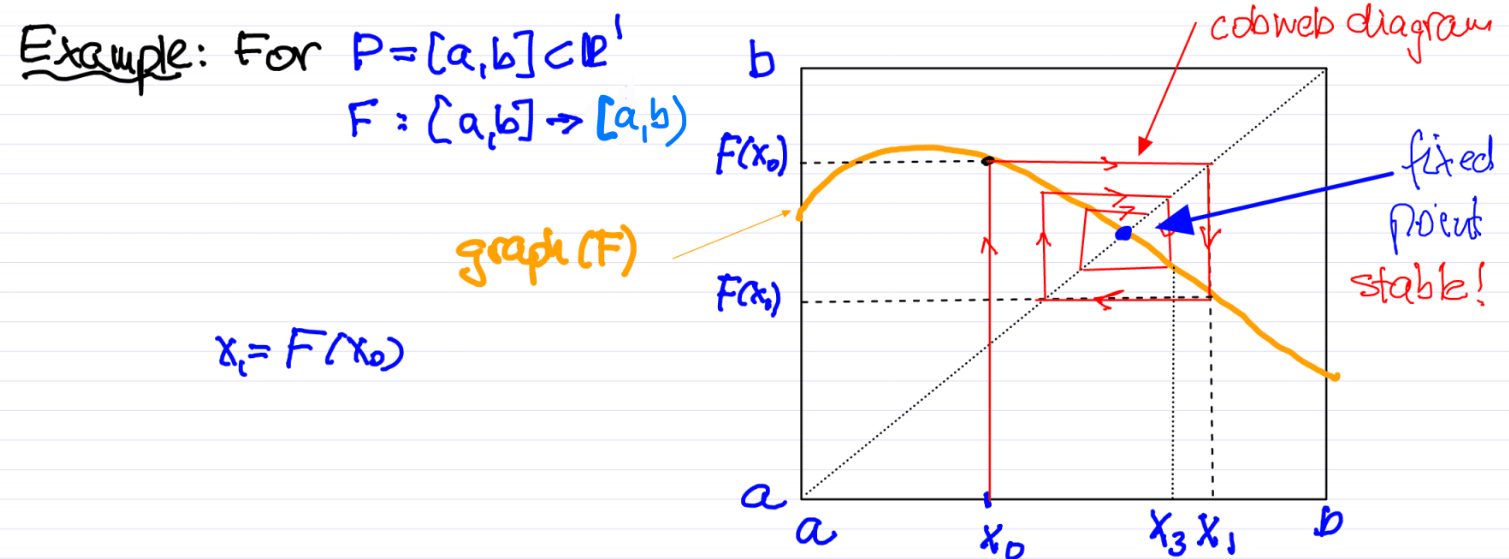
\includegraphics[width = \textwidth]{figures/intro/1DDS.png}
\end{figure}
\end{ex}

\item In a CDS we have a first order system of ordinary differential equations (ODE)
	\begin{align}
		\boxed{
			\dot{x} = f(x,t)
		}
	\end{align}
	for $x\in P$ and $t \in E$. This yields the initial value problem (IVP):
	\begin{align}
		\begin{dcases}
			\dot{x} = f(x,t) \\
			x(t_0) = x_0
		\end{dcases}
	\end{align}
	\begin{figure}[h]
	\centering
	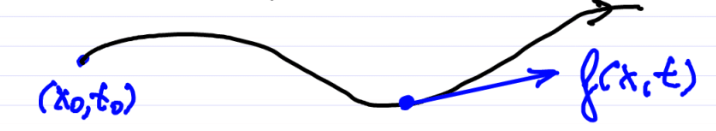
\includegraphics[width = 0.8\textwidth]{figures/intro/2CDS.png}
	\end{figure}
	
	Assuming there exists a unique solution $\varphi(t; t_0, x_0)$ with $\dot{\varphi} = f(\phi,t)$ and $\varphi(t_0)= x_0$, then the following flow map is well defined
	\begin{align}
		\boxed{
		F_{t_0}^{t}(x_0) := \varphi(t; t_0, x_0).}
	\end{align}
	Such an $F_{t_0}^{t}$ has nice properties
	\begin{itemize}
		\item $F_{t_0}^{t}$ is as smooth as $f(x,t)$,
		\item $F_{t_0}^{t_0} = I$ and $F_{t_0}^{t_2} = F_{t_1}^{t_2} \circ F_{t_0}^{t_1}$ (group property),
		\item $\left(F_{t_0}^{t}\right)^{-1} = F_{t}^{t_0}$ exists and is smooth.
\end{itemize}
A special case of this is the autonomous system 
\begin{align}
	\boxed{\dot{x} = f(x).}	
\end{align}
The autonomy of a system implies
\begin{align}
	x(s,t_0, x_0) = x(\underbrace{s-t_0}_{t}, 0, x_0) \stackrel{!}{=} x(t,x_0).
\end{align}
And the induced flow map in this case is the one-parameter family of maps
\begin{align}
	\boxed{ F^{t} = F_{0}^{t}: x_0 \mapsto x(t,x_0).}
\end{align}
\end{enumerate}
\begin{ex}[Logisitic Equation]
	For a resource-limited population, we have the following dynamic system for $a> 0$, $b> 0$, and the population $x\in \mathbb{R}_+ \cup \{0\}$
	\begin{align}
		\dot{x} = ax(b-x).
	\end{align}
	In this case we have $E=\mathbb{R}$ and $\mathcal{F} = \{F^{t}\}_{t=-\infty }^{+\infty }$. This system has globally existing unique solutions (see later).	
	\begin{figure}[h]
		\centering
		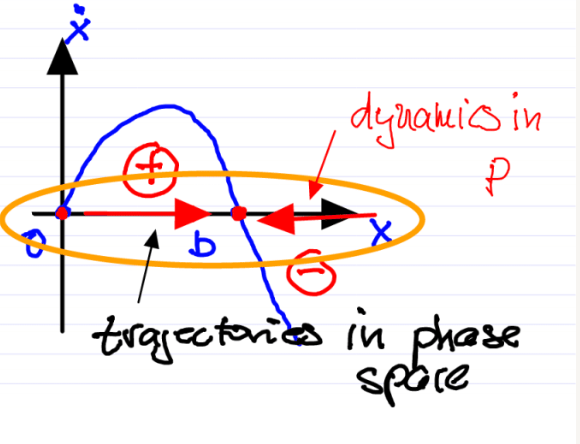
\includegraphics[width=0.4\textwidth]{figures/intro/3RHS.png}	
		\hspace{0.05\textwidth}
		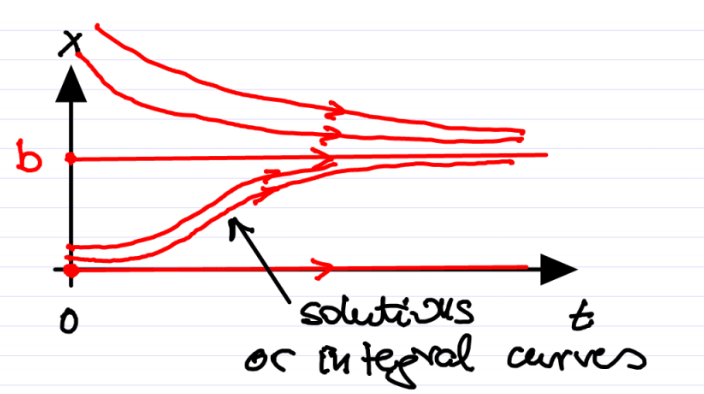
\includegraphics[width=0.4\textwidth]{figures/intro/4solutions.png}
		\caption{Left: Analysis of the right hand side. Right: Evolution in the extended phase space $P \times \mathbb{R}$.}
	\end{figure}

\end{ex}

\begin{ex}[Pendulum]
Given the equation of motion
\begin{align}
	ml^2 \ddot{\varphi} = -mgl \sin(\varphi).
\end{align}
We let $x_1 = \varphi$ and $x_2 =\dot{\varphi}$ to transform into the first-order ODE form
\begin{align}
	\begin{dcases}
		\dot{x_1} = x_2 \\
		\dot{x_2} = - \frac{g}{l} \sin (x_1).
	\end{dcases}
\end{align}
Thus we have 
\begin{align}
x = 
\begin{pmatrix}
	x_1 \\ x_2
\end{pmatrix}; \quad
f(x) = 
\begin{pmatrix}
	x_2 \\ - \frac{g}{l}\sin(x_1)	
\end{pmatrix}.
\end{align}
Qualitatively analysis gives the following facts
\begin{itemize}
	\item $x_1, x_2) = (0,0)$ and $(x_1, x_2) = (\pi , 0)$ are zeros of $f$,
	\item Energy is concerved, hence both small and large amplitude oscillations are expected,
	\item We have the symmetries $(x_1, x_2, t) \mapsto (x_1, -x_2, -t)$ and $(x_1, x_2, t) \mapsto (-x_1, x_2, -t)$.
\end{itemize}
\begin{figure}[h]
	\centering
	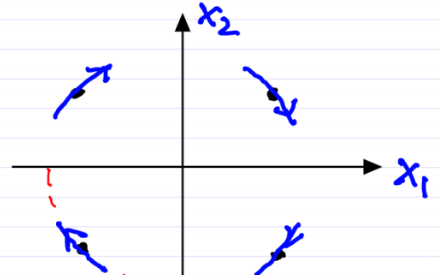
\includegraphics[width=0.4\textwidth]{figures/intro/6pendulum_symmetries.png}
	\hspace{0.05\textwidth}
	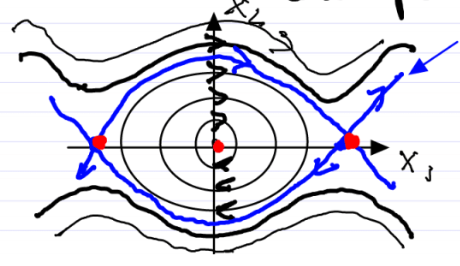
\includegraphics[width=0.4\textwidth]{figures/intro/5pendulum.png}
	\caption{Left: The symmetries of the dynamic system. Right: Phase portrait of the pendulum. The blue trajectories are separatrix.}
\end{figure}
\begin{definition}
	A separatrix connects fixed points, is unovservable by itself, and separates regions of similar behavior.
\end{definition}

\end{ex}

\begin{ex}[Exploit geometry of phase space for analysis]
	Two bikes \emph{can} make it from $A$ to $B$ on different rountes without exceeding distance $D$. Assume two trucks are trying to make it between $A$ and $B$, on different roades in teh opposite direction, carrying load of width $D$. Can the trucks make it without hitting each other?	
	\begin{figure}[h]
		\centering
		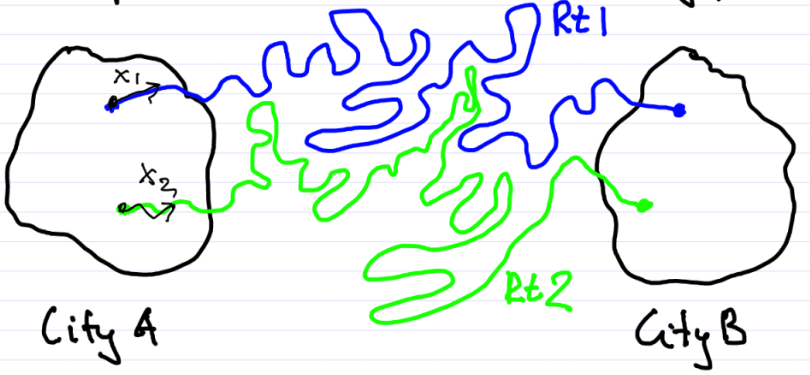
\includegraphics[width=0.5\textwidth]{figures/intro/7routes.png}
		\hspace{0.05\textwidth}
		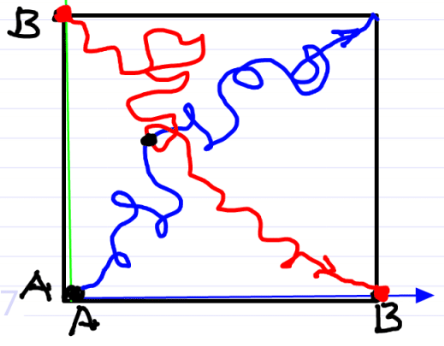
\includegraphics[width=0.3\textwidth]{figures/intro/8truck_geometry.png}
		\caption{Left: An example of the two bike routes. Right: Blue represents the phase trajectory of the two biker, red represents the phase trajectory of the two trucks.}
	\end{figure}

The two trajectories must intersect by continuity, thus at that point the trucks must be at the same positions as the bikes, implying they are within distance $D$. Therefore the trucks must crash!	
\end{ex}


